\longsection{%
  \texorpdfstring{%
    Hierarchization on Spatially Adaptive Sparse Grids\\
    with Breadth-First Search%
  }{%
    Hierarchization on Spatially Adaptive Sparse Grids
    with Breadth-First Search%
  }%
}{%
  Hierarchization on Spatially Adaptive Sparse Grids
  with Breadth-First Search%
}{%
  Hierarchization with Breadth-First Search%
}
\label{sec:44spatAdaptiveBFS}

\minitoc{87mm}{8}

\noindent
Unfortunately, we cannot apply the algorithms presented in the last
sections to spatially adaptive sparse grids with
hierarchical B-splines.
The reason is that the algorithms relied on the final interpolant $\sgintp$
being a linear combination of full grid solutions $\fgintp{\*l}$,
which is only possible for dimensionally adaptive sparse grids.
Consequently, the problem of hierarchization becomes significantly
harder if we operate on spatially adaptive sparse grids.
An exception is the case of piecewise linear basis functions ($p = 1$),
where we are still able to apply the \up,
as we will show in \cref{sec:45spatAdaptiveUP}.
%
In this section, we study one approach to hierarchize on
spatially adaptive sparse grids,
namely transforming the hierarchical basis to so-called fundamental bases
to enable a \bfs algorithm for hierarchization.

The approach in this section has already been published
\cite{Valentin18Fundamental}.
Again, note that while B-splines are our target application,
the considerations in this chapter are fully independent of the choice of
basis functions $\basis{\*l,\*i}$,
as long as they have tensor product structure.
Although we do not state it explicitly, it is possible to employ
different types of basis functions $\basis{l_t,i_t}$ in different
dimensions, e.g., B-splines of different degrees $p_t$
to enable $p$-adaptivity.



\fillsubsectionornament
\subsection{Hierarchization with Breadth-First Search on Fundamental Bases}
\label{sec:441BFSFundamentalBases}

\paragraph{Fundamental property}

As already discussed in \cref{sec:41problem},
the main cause of the difficulty of the hierarchization with B-splines
$\bspl{\*l,\*i}{p}$ is their overlapping support
(which they need for their approximation order).
Thus, high-level B-splines $\bspl{\*l',\*i'}{p}$ do not vanish
at all coarse-level grid points $\gp{\*l,\*i}$, $\*l < \*l'$.
In the univariate case,
\pagebreak%
the idea is to transform the B-spline basis to obtain
new basis functions $\fundbasis{l',i'}\colon \clint{0, 1} \to \real$
($l' \in \natz$, $i' \in \hiset{l'}$) that satisfy
\begin{subequations}
  \label{eq:fundamentalProperty}
  \begin{alignat}{3}
    \label{eq:fundamentalProperty1}
    \fundbasis{l',i'}(\centerhphantom{\gp{l,i}}{\gp{l',i}})
    &= 0,\qquad
    &&l < l',\quad
    &&i \in \hiset{l},\\
    \label{eq:fundamentalProperty2}
    \fundbasis{l',i'}(\gp{l',i})
    &= \kronecker{i}{i'},\qquad
    &&&&i \in \hiset{l'}.
  \end{alignat}
\end{subequations}
We call \eqref{eq:fundamentalProperty} \term{fundamental property}
and functions $\fundbasis{l',i'}$
that fulfill this property \term{fundamental basis functions.}
The first \cref{eq:fundamentalProperty1} ensures that
basis functions of level $l'$ vanish at
grid points of coarser levels $l < l'$.
The second \cref{eq:fundamentalProperty2} requires the
basis functions $\fundbasis{l',i'}$
to additionally vanish at all grid points of the same level $l'$
with different index $i \not= i'$.
An example for fundamental basis functions are
the piecewise linear B-splines $\bspl{l',i'}{1}$
or the Lagrange polynomials $\lagrangepoly{l',i'}$
(see \cref{fig:fundamentalProperty}, left).
The statement that $\fundbasis{l',i'}(\gp{l',i'})$ should equal one
is not an additional restriction, if
the value $\fundbasis{l',i'}(\gp{l',i'})$ is non-zero,
since we can just replace $\fundbasis{l',i'}$ with
$\fundbasis{l',i'}/\fundbasis{l',i'}(\gp{l',i'})$ to obtain
$\fundbasis{l',i'}(\gp{l',i'}) = 1$.

\begin{SCfigure}
  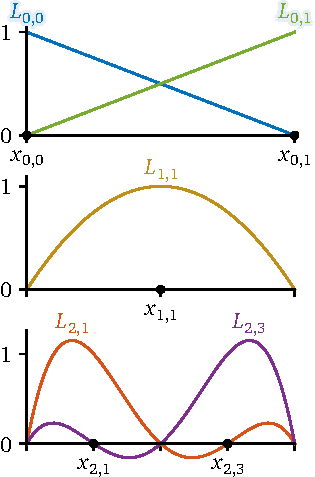
\includegraphics{hierarchicalBasis_13}\quad%
  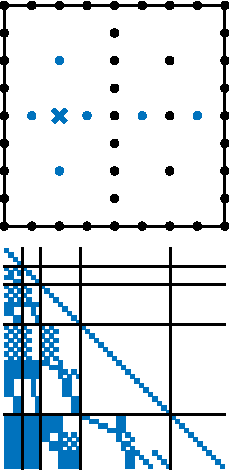
\includegraphics{matrixDensityPattern_2}%
  \caption[%
    Fundamental property with Lagrange polynomials as fundamental basis%
  ]{%
    Fundamental property with Lagrange polynomials.\\
    \emph{Left:}
    Univariate Lagrange polynomials up to level $l = 2$.\\
    \emph{Top right:}
    Regular sparse grid $\coarseregsgset{n}{d}{1}$
    ($n = 4$, $d = 2$).
    The fundamental basis function $\fundbasis{\*l',\*i'}$ corresponding
    to the marked grid point \emph{(cross)} does not vanish
    at the \textcolor{C0}{blue points} $\gp{\*l,\*i}$
    (which satisfy \eqref{eq:fundamentalPropertyImplicationMV}).\\
    \emph{Bottom right:}
    Corresponding density pattern of $\intpmat$
    when sorting rows and columns by increasing level sum
    $\normone{\*l} = 0, \dotsc, n$ \emph{(black bars).}%
  }%
  \label{fig:fundamentalProperty}%
\end{SCfigure}

\paragraph{Multivariate case}

For the multivariate case of $d \in \nat$ dimensions,
we define as usual tensor product versions
$\fundbasis{\*l',\*i'}$ of the univariate fundamental bases
$\fundbasis{l'_t,i'_t}$ ($t = 1, \dotsc, d$).
\Cref{eq:fundamentalProperty} then implies
\begin{equation}
  \label{eq:fundamentalPropertyImplicationMV}
  \fundbasis{\*l',\*i'}(\gp{\*l,\*i}) \not= 0
  \implies
  \falarge{t = 1, \dotsc, d}{
    \bracket*{(l'_t < l_t) \lor ((l'_t, i'_t) = (l_t, i_t))}
  },\quad
  (\*l, \*i), (\*l',\*i') \in \liset.
  \hspace*{-1mm}
\end{equation}
This means that every basis function
$\fundbasis{\*l',\*i'}$ can only be non-zero
at the grid points $\gp{\*l,\*i}$ that, in every dimension $t$,
have a strictly higher level $l_t$ or
the same level-index pair $(l_t, i_t)$ as the basis function.
We show an example for this relation in
\cref{fig:fundamentalProperty} (top right).

\paragraph{Triangular interpolation matrix}

The main motivation for enforcing the fundamental property
is the fact that it results in the hierarchization matrix $\intpmat$
being triangular, if the rows and columns are arranged
in the order of monotonously increasing level sum:
We assume that $k = k(\*l, \*i) \in \{1, \dotsc, N\}$ is a single
continuously enumerated index of the level-index pairs $(\*l, \*i) \in \liset$
(where $N = \setsize{\liset}$) such that
\begin{equation}
  k(\*l, \*i) \le k(\*l', \*i') \implies \normone{\*l} \le \normone{\*l'},\quad
  (\*l, \*i), (\*l', \*i') \in K,
\end{equation}
i.e., we sort the row indices $k = k(\*l, \*i)$ and
the column indices $k' = k(\*l', \*i')$ of $\intpmat$
by level sum $\normone{\cdot}$.
Consequently,
$\intpmat = (\intpmatentry{k}{k'})_{k=1,\dotsc,N,\, k'=1,\dotsc,N}$
is in lower block-triangular form:
\begin{subequations}
  \label{eq:fundamentalTriangularMV}
  \begin{alignat}{2}
    \intpmatentry{k}{k'}
    &= \fundbasis{k'}(\vgp{k})
    = 0,\quad
    &\normone{\*l}
    &< \normone{\*l'},\\
    \intertext{%
      as $\normone{\*l} < \normone{\*l'} \implies \ex{t}{l_t < l'_t}$
      and using \eqref{eq:fundamentalProperty1}.
      Additionally, the diagonal blocks are unit matrices due to%
    }
    \intpmatentry{k}{k'}
    &= \fundbasis{k'}(\vgp{k})
    \overset{(\ast)}{=} \kronecker{(\*l,\*i)}{(\*l',\*i')},\quad
    &\normone{\*l}
    &= \normone{\*l'},
  \end{alignat}
\end{subequations}
since $\normone{\*l} = \normone{\*l'}$ implies that
either $\bracket*{\ex{t}{l_t < l'_t}}$ or $\*l = \*l'$.%
\footnote{%
  Note that as specified in the list of symbols at the beginning
  of this thesis, the Kronecker delta $\kronecker{X}{Y}$
  is defined for arbitrary objects $X$ and $Y$
  that can be compared with ``$=$.''%
}
In the former case, both sides of $(\ast)$ vanish
(according to \eqref{eq:fundamentalProperty1}),
and in the latter case,
both sides equal $\kronecker{\*i}{\*i'}$
(according to \eqref{eq:fundamentalProperty2}).
Hence, $\intpmat$ is a lower-triangular matrix.
This is visualized for a two-dimensional example in
\cref{fig:fundamentalProperty} (bottom right).

\paragraph{Forward substitution}

The triangular structure of $\intpmat$ implies that
we can determine the surpluses $\surplus{\*l,\*i}$
via forward substitution:

\begin{lemma}[forward substitution]
  \label{lemma:forwardSubstitution}
  The hierarchical surpluses $\surplus{\*l,\*i}$, which
  are determined by \eqref{eq:hierarchizationSLE}
  with respect to $\fundbasis{\*l,\*i}$, satisfy
  \begin{equation}
    \surplus{\*l,\*i}
    = \fcnval{\*l,\*i} -
    \largesum{\substack{(\*l',\*i')\in\liset\\\normone{\*l'} < \normone{\*l}}}
    \surplus{\*l',\*i'} \fundbasis{\*l',\*i'}(\gp{\*l,\*i}),\quad
    (\*l, \*i) \in \liset.
  \end{equation}
\end{lemma}

\begin{proof}
  The linear system \eqref{eq:hierarchizationSLE} is given by
  \begin{subequations}
    \setlength{\abovedisplayskip}{9pt}%
    \setlength{\belowdisplayskip}{9pt}%
    \begin{align}
      \fcnval{\*l,\*i}
      &= \largesum{(\*l',\*i') \in \liset}
      \surplus{\*l',\*i'} \fundbasis{\*l',\*i'}(\gp{\*l,\*i}),\quad
      (\*l, \*i) \in \liset.\\
      \intertext{%
        According to \eqref{eq:fundamentalTriangularMV},
        all summands with $\normone{\*l'} > \normone{\*l}$ vanish
        and from the summands with $\normone{\*l'} = \normone{\*l}$,
        only the $(\*l, \*i)$-th summand remains
        with $\fundbasis{\*l,\*i}(\gp{\*l,\*i}) = 1$:%
      }
      \cdots
      &= \surplus{\*l,\*i} +
      \largesum{\substack{(\*l',\*i')\in\liset\\\normone{\*l'} < \normone{\*l}}}
      \surplus{\*l',\*i'} \fundbasis{\*l',\*i'}(\gp{\*l,\*i}).\\[-6.4em]\notag
    \end{align}
  \end{subequations}
\end{proof}

\vspace{1em}

\paragraph{Breadth-first search}

Exploiting this lemma, we formulate
a hierarchization algorithm (see \cref{alg:BFS})
that applies forward substitution by \bfs in the \dagr of
the spatially adaptive sparse grid $\sgset$.
The nodes of the \dagr are the level-index pairs $(\*l, \*i) \in \liset$.
An edge connects $(\*l, \*i)$ to $(\*l', \*i')$,
if $(\*l, \*i)$ is a direct ancestor of $(\*l', \*i')$, i.e., if
{%
  \setlength{\abovedisplayskip}{9pt}%
  \setlength{\belowdisplayskip}{9pt}%
  \begin{equation}
    \label{eq:directAncestor}
    \exlarge{t = 1, \dotsc, d}{
      \*l'_{-t} = \*l^{}_{-t},\;
      \*i'_{-t} = \*i^{}_{-t},\;
      l'_t = l^{}_t + 1,\;
      i'_t \in
      \begin{cases}
        \{1\},&l_t = 0,\\
        \{2i_t - 1, 2i_t + 1\},&l_t > 0.
      \end{cases}
    }
  \end{equation}%
}%
An example for the resulting \dagr for a regular sparse grid
in two dimensions is shown in \cref{fig:DAG}.
%
\begin{algorithm}
  \begin{algorithmic}[1]
    \Function{$\vlinout = \texttt{breadthFirstSearch}$}{%
      $\vlinin$, $\liset$%
    }
      \State{$\vlinout \gets \vlinin$}
      \label{line:algBFS3}
      \State{$K_\mathrm{p} \gets \{\*0\} \times \{0, 1\}^d$}
      \Comment{set of processed points}%
      \State{%
        $Q \gets \text{FIFO queue initialized with contents of } K_\mathrm{p}$%
      }
      \Comment{points to be processed}%
      \While{$Q \not= \emptyset$}
        \State{$(\*l', \*i') \gets Q.\pop()$}
        \Comment{obtain next point}%
        \For{%
          $\{(\*l, \*i) \in \liset \setminus \{(\*l', \*i')\} \mid
          \fa{t=1,\dotsc,d}{(l'_t < l_t) \lor ((l'_t, i'_t) = (l_t, i_t))}\}$%
        }
        \label{line:algBFS1}
          \State{%
            $\linout{\*l,\*i} \gets \linout{\*l,\*i} -
            \linout{\*l',\*i'} \fundbasis{\*l',\*i'}(\gp{\*l,\*i})$%
          }
          \Comment{%
            update surpluses according to \cref{lemma:forwardSubstitution}%
          }%
          \label{line:algBFS2}
        \EndFor{}
        \For{%
          $\{(\*l, \*i) \in \liset \setminus \liset_\mathrm{p} \mid
          \text{$(\*l, \*i)$ direct child of $(\*l', \*i')$}\}$%
        }
          \State{$Q.\push((\*l, \*i))$}
          \Comment{add children to queue}%
          \State{%
            $\liset_\mathrm{p} \gets
            \liset_\mathrm{p} \cup \{(\*l, \*i)\}$%
          }
          \Comment{mark as processed}%
        \EndFor{}
      \EndWhile{}
    \EndFunction{}
  \end{algorithmic}
  \caption[%
    Hierarchization with breadth-first search (BFS)%
  ]{%
    Hierarchization with breadth-first search
    on spatially adaptive sparse grids with fundamental bases.
    Inputs are
    the vector $\vlinin = (\linin{\*l,\*i})_{(\*l,\*i) \in \liset}$
    of input data (function values $\fcnval{\*l,\*i}$ at the grid points) and
    the set $\liset$ of level-index pairs of the
    sparse grid (see \eqref{eq:spatiallyAdaptiveSG}).
    The output is the vector
    $\vlinout = (\linout{\*l,\*i})_{(\*l,\*i) \in \liset}$
    of output data (hierarchical surpluses $\surplus{\*l,\*i}$).%
  }%
  \label{alg:BFS}%
\end{algorithm}
%
\begin{SCfigure}
  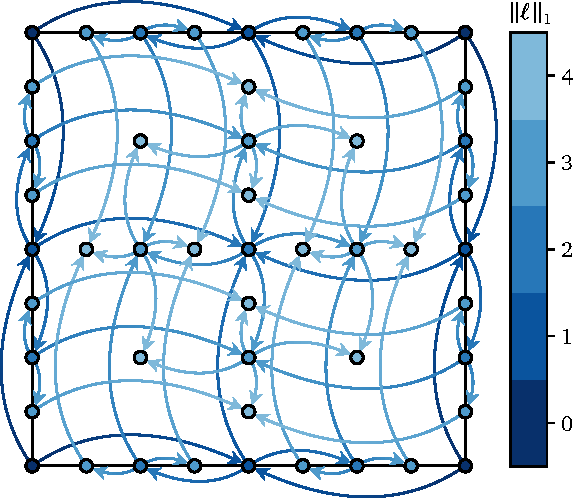
\includegraphics{dag_1}%
  \caption[%
    Sparse grid as directed acyclic graph%
  ]{%
    Ancestor relationships \emph{(arrows)} in a
    regular sparse grid $\coarseregsgset{n}{d}{1}$ \emph{(points)}
    of level $n = 4$ and dimensionality $d = 2$.
    The color indicates the level sum $\normone{\*l}$.
    Breadth-first search, as implemented in \cref{alg:BFS},
    visits all grid points $\gp{\*l,\*i}$ with level sum
    $\normone{\*l} = 0$ first,
    then those with $\normone{\*l} = 1$, and so on.%
  }%
  \label{fig:DAG}%
\end{SCfigure}
%
We make two assumptions for \cref{alg:BFS}.
First, $\liset$ should contain at least all $2^d$ corners of the
domain $\clint{\*0, \*1}$:
\begin{subequations}
  \label{eq:BFSAssumptions}
  \begin{equation}
    \label{eq:BFSAssumption1}
    \liset \supset \{\*0\} \times \{0, 1\}^d
    = \{(\*0, \*i) \mid \*i \in \{0, 1\}^d\}.
  \end{equation}
  Second, all grid points should be reachable from the corners:
  \begin{equation}
    \label{eq:bfsAssumption2}
    \begin{split}
      \forall_{(\*l', \*i') \in \liset}
      \exists_{m \in \natz}
      \exists_{
        (\*l^{(0)}, \*i^{(0)}), \dotsc, (\*l^{(m)}, \*i^{(m)}) \in \liset
      }\;\;
      &\bigl[(\*l^{(0)}, \*i^{(0)}) \to \dotsb \to (\*l^{(m)}, \*i^{(m)}),\\
      &\hspace{3mm} \*l^{(0)} = \*0,\;
      (\*l^{(m)}, \*i^{(m)}) = (\*l', \*i')\bigr],
    \end{split}
  \end{equation}
\end{subequations}
where ``$\to$'' is the direct ancestor relation \eqref{eq:directAncestor}.
One can also use a different initial set than the corners
of $\clint{\*0, \*1}$, e.g., when working with sparse grids
without boundary points.
In general, there are three requirements on the initial set:
First, all grid points should be reachable from this set.
Second, the grid points in the set are sorted by increasing level sum
(if the set contains grid points with different level sums).
Third, the surpluses corresponding to the initial grid points
need to be precalculated correctly
before the \texttt{\algorithmicwhile} loop in \cref{alg:BFS}.

\paragraph{Correctness}

The correctness of \cref{alg:BFS} can be shown with the following invariant:

\begin{restatable}[invariant of breadth-first-search hierarchization]{%
  proposition%
}{%
  propInvariantBFS%
}
  \label{prop:invariantBFS}
  Under the assumption \eqref{eq:BFSAssumptions},
  it holds after \pop{}\,ping all grid points with level sum $< q$
  from the queue $Q$ in \cref{alg:BFS}:
  \begin{equation}
    \label{eq:propInvariantBFS}
    \linout{\*l,\*i}
    = \fcnval{\*l,\*i} -
    \largesum{\substack{(\*l',\*i')\in\liset\\\normone{\*l'} < q}}
    \linout{\*l',\*i'} \fundbasis{\*l',\*i'}(\gp{\*l,\*i}),\quad
    (\*l, \*i) \in \liset,\;\;
    \normone{\*l} = q.
    \hspace*{-6mm}
  \end{equation}
\end{restatable}

\vspace{-0.8em}

\begin{proof}
  See \cref{sec:a133proofBFS}.
\end{proof}

\vspace{0.8em}

\begin{shortcorollary}[correctness of breadth-first-search hierarchization]
  \label{cor:algBFSCorrectness}
  \Cref{alg:BFS} is correct.
\end{shortcorollary}

\begin{proof}
  As noted in the proof of \cref{prop:invariantBFS},
  the result $\linout{\*l,\*i}$ after \pop{}ping all grid points with level sum
  $q$ as stated in \cref{prop:invariantBFS} is also the final result
  of the algorithm:
  \begin{equation}
    \linout{\*l,\*i}
    = \fcnval{\*l,\*i} -
    \largesum{\substack{(\*l',\*i')\in\liset\\\normone{\*l'} < \normone{\*l}}}
    \linout{\*l',\*i'} \fundbasis{\*l',\*i'}(\gp{\*l,\*i}),\quad
    (\*l, \*i) \in \liset.
  \end{equation}
  By \cref{lemma:forwardSubstitution},
  the correct hierarchical surpluses $\surplus{\*l,\*i}$
  satisfy the same relation.
  Inductively, $\linout{\*l,\*i}$ and $\surplus{\*l,\*i}$ must coincide.
\end{proof}

\paragraph{Complexity}

The \bfs algorithm in \cref{alg:BFS} is not as efficient as the \up:
It still needs to perform $\landauO{N^2 d}$ many univariate
basis evaluations (compared to $\landauO{Nd}$ for the \up).
However, it only needs linear space $\landauO{N}$ similar to the
\up\punctfix{.}
This is a significant advantage over directly solving the system
\eqref{eq:hierarchizationSLE} of linear equations, which typically
needs quadratic space $\landauO{N^2}$.



\subsection{Constructing Fundamental Bases}
\label{sec:442constructingFundamentalBases}

Unfortunately, the hierarchical B-splines $\bspl{l',i'}{p}$ do not
satisfy the fundamental property \eqref{eq:fundamentalProperty}.
We now focus on the construction of univariate fundamental bases
$\fundbasis{l',i'}$ starting from an
arbitrary hierarchical basis $\basis{l',i'}$.
To this end, we study two transformations
$\basis{l',i'} \mapsto \fundbasis{l',i'}$.
As usual, the multivariate case is treated with the
tensor product approach.

\paragraph{Hierarchical fundamental transformation (HFT)}

The canonical way to find a fundamental basis $\fundbasis{l',i'}$ is to
use a linear combination $\basis[\hft]{l',i'}$
of coarser basis functions $\basis{l'',i''}$ as an ansatz
and require that the fundamental property \eqref{eq:fundamentalProperty}
is fulfilled:
\begin{equation}
  \label{eq:hierarchicalFundamentalTransformation}
  \basis[\hft]{l',i'}
  \ceq \sum_{l''=0}^{l'} \sum_{i'' \in \hiset{l''}}
  c_{l'',i''}^{l',i'} \basis{l'',i''}
  \quad\text{such that}\quad
  \fafalarge{l = 0, \dotsc, l'}{i \in \hiset{l}}{
    \basis[\hft]{l',i'}(\gp{l,i}) = \kronecker{(l,i)}{(l',i')}.
  }
\end{equation}
This means that
$\basis[\hft]{l',i'}$ ($l' \in \natz$, $i' = 0, \dotsc, 2^{l'}$)
interpolates the data
$\{(\gp{l',i}, \kronecker{i}{i'}) \mid i = 0, \dotsc, 2^{l'}\}$.
The coefficients $c_{l'',i''}^{l',i'} \in \real$
are, in general, different for each basis function $\basis[\hft]{l',i'}$.
This complicates precomputation and storage of the $2^{l'} + 1$ coefficients,
as they have to be determined by solving a system of linear equations.
In addition, the transformation $\basis{l',i'} \mapsto \basis[\hft]{l',i'}$
does not preserve the locality of the support of the basis functions.
Consequently, $\basis[\hft]{l',i'}$ may be globally supported,
which means that we have to evaluate up to $2^{l'} + 1$ basis functions
$\basis{l'',i''}$ when evaluating $\basis[\hft]{l',i'}$ at a single point
$x \in \clint{0, 1}$.
The global support of the resulting transformed basis
for uniform hierarchical B-splines (which are locally supported)
can be seen in \cref{fig:hftBSpline}.

\begin{SCfigure}
  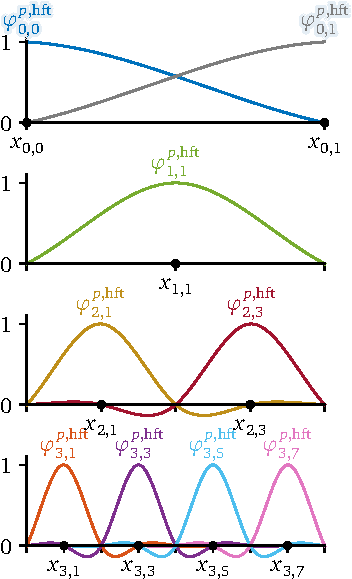
\includegraphics{hierarchicalBasis_14}%
  \caption[%
    Hierarchical fundamental transformation on hierarchical B-splines%
  ]{%
    Resulting basis functions $\bspl[\hft]{l',i'}{p}$
    ($l' \le l$, $i' \in \hiset{l'}$)
    after applying the hierarchical fundamental transformation
    to hierarchical cubic B-splines ($p = 3$) and
    grid points $\gp{l',i'}$ \emph{(dots)} up to level $l = 3$.%
  }%
  \label{fig:hftBSpline}%
\end{SCfigure}

We call the transformation $\basis{l',i'} \mapsto \basis[\hft]{l',i'}$
\term{\hftr.}
The following proposition shows that this is only a change of basis,
as the spanned sparse grid space remains unchanged.
While the proposition is formulated for regular sparse grids,
a similar statement can be proven for the dimensionally adaptive case.

\begin{proposition}[%
  spanned sparse grid space for the HFT%
]
  \label{prop:hftSparseGridSpace}
  If $\liset \ceq \{(\*l, \*i) \mid
  \normone{\*l'} \le n,\; \*i' \in \hiset{\*l'}\}$
  is the set of level-index pairs for the regular sparse grid of level $n$
  and dimensionality $d$, then
  \begin{equation}
    \regsgspace{n}{d}
    = \regsgspace[\hft]{n}{d}
    \ceq \spn\{\basis[\hft]{\*l',\*i'} \mid (\*l', \*i') \in \liset\}.
  \end{equation}
\end{proposition}

\begin{proof}
  We have $\regsgspace{n}{d} \supset \regsgspace[\hft]{n}{d}$ as
  $\basis[\hft]{\*l',\*i'} \in \regsgspace{n}{d}$
  for all $(\*l', \*i') \in \liset$:
  \begin{equation}
    \basis[\hft]{\*l',\*i'}
    = \prod_{t=1}^d \, \sum_{l''_t=0}^{l'_t} \, \sum_{i''_t \in \hiset{l''_t}}
    c_{l''_t,i''_t}^{l'_t,i'_t} \basis{l''_t,i''_t}
    = \sum_{\*l''=\*0}^{\*l'} \, \sum_{\*i'' \in \hiset{\*l''}}
    c_{\*l'',\*i''}^{\*l',\*i'} \basis{\*l'',\*i''}
    \in \regsgspace{n}{d},\quad
    c_{\*l'',\*i''}^{\*l',\*i'}
    \ceq \prod_{t=1}^d c_{l''_t,i''_t}^{l'_t,i'_t}.
  \end{equation}
  
  To prove that $\regsgspace{n}{d} \subset \regsgspace[\hft]{n}{d}$,
  we show that the dimension of $\regsgspace[\hft]{n}{d}$
  matches $\dim \regsgspace{n}{d} = \setsize{\liset}$.
  It suffices to show that
  the functions $\basis[\hft]{\*l',\*i'}$ ($(\*l', \*i') \in \liset$),
  are linearly independent.
  Let $\surplus{\*l',\*i'} \in \real$ be with
  $\sum_{(\*l', \*i') \in \liset}
  \surplus{\*l',\*i'} \basis[\hft]{\*l',\*i'} \equiv 0$.
  By evaluating at $\gp{\*l,\*i}$ ($(\*l, \*i) \in \liset$), we obtain
  \begin{equation}
    \largesum{(\*l', \*i') \in \liset}
    \surplus{\*l',\*i'} \basis[\hft]{\*l',\*i'}(\gp{\*l,\*i}) = 0,\quad
    (\*l, \*i) \in \liset.
  \end{equation}
  This is a lower triangular system according to
  \eqref{eq:fundamentalTriangularMV},
  which implies $\surplus{\*l',\*i'} = 0$ for all $(\*l, \*i) \in \liset$.
  Hence, the functions $\basis[\hft]{\*l',\*i'}$ ($(\*l', \*i') \in \liset$)
  are linearly independent.
\end{proof}

\paragraph{Translation-invariant fundamental transformation (TIFT)}

Another disadvantage of the \hftr is that it does not preserve
the so-called \term{translation invariance} of the original basis.
A~basis $\basis{l,i}$ ($l \in \natz$, $i = 0, \dotsc, 2^l$)
is translation-invariant, if there is a \term{parent function}
$\parentfcn\colon \real \to \real$
such that
\begin{equation}
  \label{eq:translationInvariance}
  \basis{l,i}(x)
  = \parentfcn(\tfrac{x}{\ms{l}} - i),\quad
  l \in \natz,\;\;
  i = 0, \dotsc, 2^l,\;\;
  x \in \clint{0, 1}.
\end{equation}
The fact that the \hftr does not preserve translation invariance means
that for each basis function $\basis[\hft]{l',i'}$, we have to
calculate its individual $2^{l'} + 1$ coefficients $c_{l'',i''}^{l',i'}$.

To solve this problem,
we use a similar ansatz as for the \hftr,
but we replace the hierarchical basis functions $\basis{l'',i''}$
($l'' = 0, \dotsc, l'$,\, $i'' \in \hiset{l''}$)
with nodal basis functions $\basis{l',i''}$ and
allow general integer indices $i'' \in \integer$:
\begin{equation}
  \label{eq:tiftDefinition}
  \basis[\tift]{l',i'}
  \ceq \sum_{i'' \in \integer} c_{i''}^{l',i'} \basis{l',i''}
  \quad\text{such that}\quad
  \falarge{i \in \hiset{l'}}{
    \basis[\tift]{l',i'}(\gp{l',i}) = \kronecker{i}{i'},
  }
\end{equation}
where $l' \in \natz$, $i' = 0, \dotsc, 2^{l'}$, and
$c_{i''}^{l',i'} \in \real$.
We have to make three assumptions for \eqref{eq:tiftDefinition} to make sense:

\begin{itemize}
  \item
  The functions $\basis{l',i''}$ have to be defined for integer indices
  $i'' \in \integer$, i.e.,
  the functions $\basis{l',i''}\colon \clint{0, 1} \to \real$
  must also exist for $i'' < 0$ or $i'' > 2^{l'}$.
  This is the case for translation-invariant bases
  $\basis{l',i''}$ (such as B-splines $\bspl{l',i''}{p}$),
  as they can be generalized to $i'' \in \integer$
  via \cref{eq:translationInvariance}.
  
  \item
  The set
  \begin{equation}
    \relindexset{l'}
    \ceq \braced*{
      i'' \in \integer \bigm\vert
      \restrictfcn{\basis{l',i''}}{\clint{0, 1}} \not\equiv 0
    },\quad
    l' \in \natz,
  \end{equation}
  of relevant indices should be finite,
  so that in each point $x \in \clint{0, 1}$
  only a finite number of basis functions $\basis{l',i''}$ of level $l'$
  is non-zero.
  This means that the series in \eqref{eq:tiftDefinition} collapses to a
  finite sum over $i'' \in \relindexset{l'}$.
  The condition is met for compactly supported and translation-invariant
  basis functions such as B-splines $\bspl{l',i''}{p}$.
  For $d \in \nat$ dimensions and $\*l' \in \natz^d$, we define
  $\relindexset{\*l'} \ceq
  \relindexset{l'_1} \times \dotsb \times \relindexset{l'_d}$.
  
  \item
  The coefficients $c_{i''}^{l',i'}$, such that
  \eqref{eq:tiftDefinition} holds, exist and are uniquely determined.
\end{itemize}

\vspace{1em}

\noindent
Let $\basis{l',i''}$ be translation-invariant and
let $l' \in \natz$ and $i' = 0, \dotsc, 2^{l'}$ be arbitrary.
Then we have
\begin{equation}
  \label{eq:tiftParentFunctionDerivation}
  \basis[\tift]{l',i'}(x)
  = \sum_{i'' \in \integer} c_{i''}^{l',i'} \basis{l',i''}(x)
  \!\overset{\eqref{eq:translationInvariance}}{=}\!
  \sum_{i'' \in \integer} c_{i''}^{l',i'}
  \parentfcn(\tfrac{x}{\ms{l'}} - i'')
  = \sum_{i'' \in \integer}
  c_{i'+i''}^{l',i'} \parentfcn((\tfrac{x}{\ms{l'}} - i') - i''),
\end{equation}
where the function defined by
$\sum_{i'' \in \integer} c_{i'+i''}^{l',i'} \parentfcn({\cdot} - i'')$
satisfies
\begin{subequations}
  \label{eq:tiftParentFunctionConditions}
  \begin{align}
    \sum_{i'' \in \integer} c_{i'+i''}^{l',i'} \parentfcn(i - i'')
    &= \sum_{i'' \in \integer} c_{i'+i''}^{l',i'}
    \parentfcn((\tfrac{\gp{l',i+i'}}{\ms{l'}} - i') - i'')
    \!\overset{\eqref{eq:tiftParentFunctionDerivation}}{=}\!
    \basis[\tift]{l',i'}(\gp{l',i+i'})
    \!\overset{\eqref{eq:tiftDefinition}}{=}\!
    \kronecker{i'}{i+i'}\\
    &= \kronecker{i}{0},\quad
    i \in \integer.
  \end{align}
\end{subequations}
Due to the translation invariance and the third assumption in the list above,
there is only a single set of coefficients of $\parentfcn({\cdot} - i'')$
such that \eqref{eq:tiftParentFunctionConditions} holds.
This means that $c_{i'+i''}^{l',i'}$ does not depend on $l'$ or $i'$,
if $\basis{l',i'}$ is translation-invariant.
Consequently, if we set $c_{i''} \ceq c_{i'+i''}^{l',i'}$
for some arbitrary $l' \in \natz$ and $i' = 0, \dotsc, 2^{l'}$,
then $\parentfcn[\tift]\colon \real \to \real$ defined by
\begin{equation}
  \label{eq:tiftParentFunctionDefinition}
  \parentfcn[\tift](x)
  \ceq \sum_{i'' \in \integer} c_{i''} \parentfcn(x - i''),\quad
  x \in \clint{0, 1},
\end{equation}
is a parent function of $\basis[\tift]{l',i'}$ that satisfies
\begin{equation}
  \label{eq:tiftParentFunctionInterpolation}
  \falarge{i \in \integer}{
    \parentfcn[\tift](i) = \kronecker{i}{0}.
  }
\end{equation}
The fact that $\parentfcn[\tift]$ is the parent function of
$\basis[\tift]{l',i'}$ easily follows from
\eqref{eq:tiftParentFunctionDerivation}
as the \rhs is exactly $\parentfcn[\tift](\tfrac{x}{\ms{l'}} - i')$,
as required by \eqref{eq:translationInvariance}.
This shows that the transformation $\basis{l',i'} \mapsto \basis[\tift]{l',i'}$
preserves translation-invariance.
Therefore, we call the transformation
$\basis{l',i'} \mapsto \basis[\tift]{l',i'}$ \term{\tiftr.}

\vspace{2em}

In contrast to the \hftr, the \tiftr is only a change of basis
if we consider the extended nodal spaces that also include
basis functions with indices outside $\{0, \dotsc, 2^{l'}\}$.
This is the statement of the following proposition
(generalized to the $d$-variate case).
Note that although the proposition involves basis functions
$\basis{\*l',\*i'}$ and $\basis[\tift]{\*l',\*i'}$
outside the domain $\clint{0, 1}$
(in the sense that $\gp{\*l',\*i'} \notin \clint{0, 1}$),
we still restrict all functions to $\clint{0, 1}$.
We cannot formulate an equivalent version of \thmref{prop:hftSparseGridSpace},
as it might be that, in one dimension,
$\basis{l',i''}$ ($i'' < 0$ or $i'' > 2^{l'}$)
is not contained in the nodal space $\ns{l'}$.

\pagebreak

\begin{proposition}[%
  spanned nodal space for the TIFT%
]
  \label{prop:tiftNodalSpace}
  We have
  \begin{equation}
    \hspace*{-10mm}
    \spn\{\basis{\*l',\*i'} \mid \*i' \in \relindexset{\*l'}\}
    =: \ns[\ext]{\*l'}
    = \ns[\tift,\ext]{\*l'}
    \ceq \spn\{\basis[\tift]{\*l',\*i'} \mid \*i' \in \relindexset{\*l'}\},\quad
    \*l' \in \natz^d.
    \hspace*{-20mm}
  \end{equation}
\end{proposition}

\vspace{1em}

\begin{proof}
  We have $\ns[\ext]{\*l'} \supset \ns[\tift,\ext]{\*l'}$ as
  $\basis[\tift]{\*l',\*i'} \in \ns[\ext]{\*l'}$
  for all $\*i' \in \relindexset{\*l'}$:
  \begin{equation}
    \basis[\tift]{\*l',\*i'}
    = \prod_{t=1}^d \sum_{i''_t \in \relindexset{l'_t}}
    c_{i''_t}^{l'_t,i'_t} \basis{l'_t,i''_t}
    = \sum_{\*i'' \in \relindexset{\*l'}}
    c_{\*i''}^{\*l',\*i'} \basis{\*l',\*i''}
    \in \ns[\ext]{\*l'},\quad
    c_{\*i''}^{\*l',\*i'}
    \ceq \prod_{t=1}^d c_{i''_t}^{l'_t,i'_t}.
  \end{equation}
  
  To prove that
  $\ns[\ext]{\*l'} \subset \ns[\tift,\ext]{\*l'}$,
  we show that the dimensions of the two spaces match.
  As before, it suffices to show that
  the functions $\basis[\tift]{\*l',\*i'}$ ($\*i' \in \relindexset{\*l'}$)
  are linearly independent.
  Let $\surplus{\*l',\*i'} \in \real$ be with
  $\sum_{\*i' \in \relindexset{\*l'}}
  \surplus{\*l',\*i'} \basis[\tift]{\*l',\*i'} \equiv 0$.
  By evaluating at $\gp{\*l',\*i}$ ($\*i \in \relindexset{\*l'}$), we obtain
  \begin{equation}
    0
    = \sum_{\*i' \in \relindexset{\*l'}} \surplus{\*l',\*i'}
    \underbrace{\basis[\tift]{\*l',\*i'}(\gp{\*l',\*i})}_{=\kronecker{\*i}{\*i'}}
    = \surplus{\*l',\*i},\quad
    \*i \in \relindexset{\*l'},
  \end{equation}
  i.e., all coefficients $\surplus{\*l',\*i'}$ must vanish.%
  \footnote{%
    Note that we have to allow evaluations outside the
    domain $\clint{0, 1}$ for this step.
    However, this is feasible for proving the linear independence
    of $\basis[\tift]{\*l',\*i'}$, since we can just restrict the functions
    after showing that the extended nodal spaces equal.%
  }
  Hence, the functions $\basis[\tift]{\*l',\*i'}$ ($\*i' \in \relindexset{\*l'}$)
  are linearly independent.
\end{proof}



\fillsubsectionornament
\subsection{Hierarchical Fundamental Splines}
\label{sec:443fundamentalSplines}

\paragraph{Definition}

We now apply the translation-invariant fundamental transformation
to hierarchical B-splines $\bspl{l,i}{p}$ of degree $p$.
The parent function $\parentbspl{p}\colon \real \to \real$ of B-splines
and the set $\relindexset[p]{l}$ of relevant indices for level $l \in \natz$
are given by
\begin{equation}
  \parentbspl{p}(x)
  \ceq \cardbspl{p}(x + \tfrac{p+1}{2}),\qquad
  \relindexset[p]{l}
  \ceq \{-\tfrac{p-1}{2},\;
  -\tfrac{p-1}{2} + 1,\;
  \dotsc,\;
  2^l + \tfrac{p-1}{2}\},
\end{equation}
respectively.
According to \eqref{eq:tiftParentFunctionInterpolation},
the coefficients $\fundsplcoeff{k}{p} \in \real$ of
the transformed parent function $\parentfcn[p,\tift]$
in \cref{eq:tiftParentFunctionDefinition} are determined by a
\pagebreak%
bi-infinite-dimensional system of linear equations:
\begin{equation}
  \label{eq:fundamentalSplineSLE}
  \newcommand*{\vala}{\cardbspl{p}(\tfrac{p+1}{2} - 2)}
  \newcommand*{\valb}{\cardbspl{p}(\tfrac{p+1}{2} - 1)}
  \newcommand*{\valc}{\cardbspl{p}(\tfrac{p+1}{2})}
  \newcommand*{\vald}{\cardbspl{p}(\tfrac{p+1}{2} + 1)}
  \newcommand*{\vale}{\cardbspl{p}(\tfrac{p+1}{2} + 2)}
  \newcommand*{\ddotsr}{\rotatebox{16}{$\ddots$}}
  \newcommand*{\raiseentry}[1]{\raisebox{0.3em}{$#1$}}
  \paren*{
    \begin{array}{%
      @{}>{\raggedright\arraybackslash$}m{14mm}<{$}@{}%
      *{3}{%
        @{}>{\centering\arraybackslash$}m{23mm}<{$}@{}%
      }%
      @{}>{\raggedleft\arraybackslash$}m{14mm}<{$}@{}%
    }
      \ddotsr&\ddotsr&\ddotsr&       &       \\
      \ddotsr&\valc  &\valb  &\vala  &       \\
      \ddotsr&\vald  &\valc  &\valb  &\ddotsr\\
             &\vale  &\vald  &\valc  &\ddotsr\\
             &       &\ddotsr&\ddotsr&\ddotsr
    \end{array}
  }
  \cdot
  \begin{pmatrix}
    \vphantom{\ddotsr}\raiseentry{\vdots}\\
    \vphantom{\ddotsr}\raiseentry{\fundsplcoeff{-1}{p}}\\
    \vphantom{\ddotsr}\raiseentry{\fundsplcoeff{0}{p}}\\
    \vphantom{\ddotsr}\raiseentry{\fundsplcoeff{1}{p}}\\
    \vphantom{\ddotsr}\raiseentry{\vdots}
  \end{pmatrix}
  =
  \begin{pmatrix}
    \vphantom{\ddotsr}\raiseentry{\vdots}\\
    \vphantom{\ddotsr}\raiseentry{0}\\
    \vphantom{\ddotsr}\raiseentry{1}\\
    \vphantom{\ddotsr}\raiseentry{0}\\
    \vphantom{\ddotsr}\raiseentry{\vdots}
  \end{pmatrix}.
\end{equation}
As in each row only $p$ entries are non-zero,
the system matrix is a symmetric banded Toeplitz matrix%
\footnote{%
  The entries $a_{k,j}$ of a Toeplitz matrix $\mat{A}$
  solely depend on $k - j$, i.e.,
  $a_{k,j} = c_{k-j}$ for some vector $\*c$.%
}.
One can show that the linear system \eqref{eq:fundamentalSplineSLE}
is uniquely solvable:

\begin{theorem}[unique existence of fundamental spline coefficients]
  \label{thm:fundamentalSplineExistence}
  \usenotation{zzzzfs}
  The system \eqref{eq:fundamentalSplineSLE} has a unique solution
  $(\fundsplcoeff{k}{p})_{k \in \integer}$ and the corresponding parent function
  $\parentfundspl{p}\colon \real \to \real$ defined by
  $\parentfundspl{p}(x) \ceq
  \sum_{k \in \integer} \fundsplcoeff{k}{p} \parentbspl{p}(x - k)$
  satisfies
  \begin{equation}
    \exfalarge{\beta_p, \gamma_p \in \posreal}{x \in \real}{
      \abs{\parentfundspl{p}(x)}
      \le \beta_p \cdot (\gamma_p)^{-\abs{x}}.
    }
  \end{equation}
\end{theorem}

\begin{proof}
  See Theorems 1 and 2 in \cite{Schoenberg72Cardinal}.
\end{proof}

The function $\parentfundspl{p}$ from \cref{thm:fundamentalSplineExistence}
is well-known as the \term{fundamental spline} of degree~$p$
\multicite{Schoenberg72Cardinal,Schoenberg73Cardinal}.
Applications of fundamental splines are interpolation and
the definition of spline wavelets \cite{Chui92Introduction}.
The fundamental splines $\parentfundspl{p}$ of low degrees $p$ and
their bounding functions $\beta_p \cdot (\gamma_p)^{-\abs{x}}$
are plotted in \cref{fig:fundamentalSpline}.

\begin{figure}
  \subcaptionbox{%
    $p = 1$%
  }[72mm]{%
    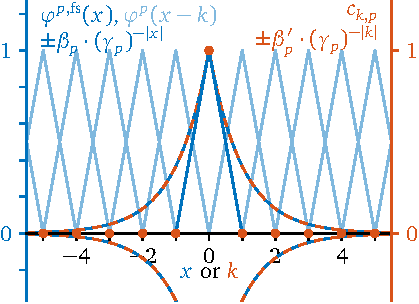
\includegraphics{fundamentalSpline_1}%
  }%
  \hfill%
  \subcaptionbox{%
    $p = 3$%
  }[72mm]{%
    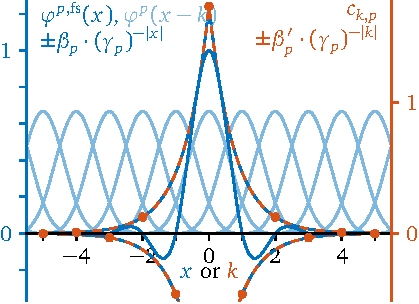
\includegraphics{fundamentalSpline_2}%
  }\\[4mm]%
  \subcaptionbox{%
    $p = 5$%
  }[72mm]{%
    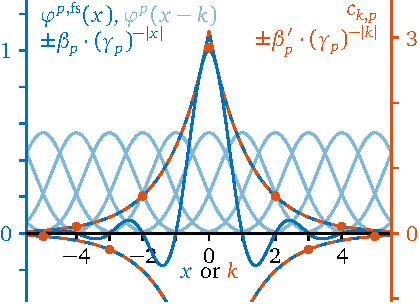
\includegraphics{fundamentalSpline_3}%
  }%
  \hfill%
  \subcaptionbox{%
    $p = 7$%
  }[72mm]{%
    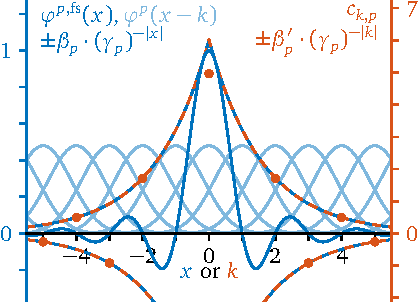
\includegraphics{fundamentalSpline_4}%
  }%
  \caption[%
    Fundamental splines and their B-spline coefficients%
  ]{%
    The fundamental spline $\parentfundspl{p}$ \emph{\textcolor{C0}{(blue)}}
    is a linear combination of cardinal B-splines $\cardbspl{p}({\cdot} - k)$,
    $k \in \integer$ \emph{\textcolor{C0!50}{(light blue)},}
    \vspace{-0.1em}%
    with coefficients $\fundsplcoeff{k}{p}$ \emph{\textcolor{C1}{(red points)}.}
    The absolute values of the fundamental spline $\parentfundspl{p}$ and
    its coefficients are bounded by a multiple of $(\gamma_p)^{-\abs{k}}$
    \emph{(\textcolor{C0}{blue}-\textcolor{C1}{red}-dashed line).}
    The axis for $\fundsplcoeff{k}{p}$ (on the right side) is scaled such that
    both bounding functions are on top of each other.%
  }%
  \label{fig:fundamentalSpline}%
\end{figure}

\paragraph{Definition of hierarchical fundamental splines}

The fundamental spline $\parentfundspl{p}$ defines
hierarchical fundamental spline functions
$\bspl[\fs]{l,i}{p}\colon \clint{0, 1} \to \real$ via
\cref{eq:translationInvariance}, i.e.,
\begin{equation}
  \bspl[\fs]{l,i}{p}(x)
  \ceq \parentfundspl{p}(\tfrac{x}{\ms{l}} - i),\quad
  l \in \natz,\;\;
  i = 0, \dotsc, 2^l,\;\;
  x \in \clint{0, 1}.
\end{equation}
The hierarchical cubic fundamental spline basis is depicted in
\cref{fig:hierarchicalFundamentalSpline}.
As usual, we define $d$-variate hierarchical fundamental splines
as tensor products of their univariate counterparts.
According to \thmref{prop:splineSpace} and \thmref{prop:tiftNodalSpace},
the common extended nodal space
$\nsbspl[\ext]{\*l}{\*p} = \nsbspl[\fs,\ext]{\*l}{\*p}$
is equal to the spline space $\wholesplspace{\*l}{\*p}$
defined by the Cartesian product of
knot sequences of the form \eqref{eq:fullGridKnots},
i.e., the space of all splines of degree $\*p$ on the full grid of level $\*l$.

\begin{SCfigure}
  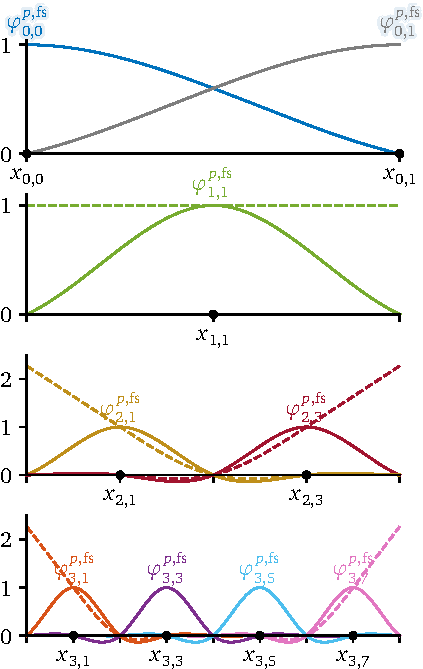
\includegraphics{hierarchicalBasis_15}%
  \caption[%
    Hierarchical fundamental splines%
  ]{%
    Hierarchical cubic fundamental splines
    $\bspl[\fs]{l',i'}{p}$
    ($l' \le l$, $i' \in \hiset{l'}$, $p = 3$),
    their modified versions $\bspl[\fs,\modified]{l',i'}{p}$
    \emph{(dashed),} and
    grid points $\gp{l',i'}$ \emph{(dots)} up to level $l = 3$.%
  }%
  \label{fig:hierarchicalFundamentalSpline}%
\end{SCfigure}

The B-spline coefficients $(\fundsplcoeff{k}{p})_{k \in \integer}$ of the
fundamental spline $\parentfundspl{p}$ decay with the same rate
as the fundamental spline itself due to the stability of the B-spline basis
\cite{Hoellig13Approximation}, i.e.,
\begin{equation}
  \label{eq:fundamentalSplineCoefficientsDecay}
  \abs{\fundsplcoeff{k}{p}}
  \le \beta'_p \cdot (\gamma_p)^{-\abs{k}},\quad
  k \in \integer,
\end{equation}
for some $\beta'_p > 0$ independent of $k$,
which is also shown in \cref{fig:fundamentalSpline}.
For $p > 1$,
there is a surprising relationship between the optimal (i.e., largest)
decay rate $\gamma_p$ and the polynomial
$\sum_{k=1}^p \cardbspl{p}(k) x^{k-1}$,
whose coefficients are the values of the
cardinal B-spline $\cardbspl{p}$ at its inner knots:
The decay rate is given by the absolute value of the largest root smaller
than $-1$ of said polynomial
(see \multicite{Chui92Introduction,Schoenberg73Cardinal}).

\vspace*{\fill}

Due to \eqref{eq:fundamentalSplineCoefficientsDecay},
we may solve the system \eqref{eq:fundamentalSplineSLE}
of linear equations approximately,
if we symmetrically truncate the linear system to
\pagebreak
$2\fundsplcutoff{p} - 1$ rows and columns
and set $\fundsplcoeff{k}{p} \ceq 0$ for all $\abs{k} \ge \fundsplcutoff{p}$,
where $\fundsplcutoff{p} \in \nat$ is a truncation index.
Note that we only have to perform $p + 1$ cardinal B-spline evaluations
to evaluate $\parentfundspl{p}$ once.
In \cref{tbl:fundamentalSplineDecay}, we list the decay rates $\gamma_p$,
the factors $\beta_p$ and $\beta'_p$, and the truncation indices
$\fundsplcutoff{p}$ for different $p$.

\begin{table}
  \setnumberoftableheaderrows{1}%
  \begin{tabular}{%
    >{\kern\tabcolsep}=l<{\kern5mm}*{8}{+c}<{\kern\tabcolsep}%
  }
    \toprulec
    \headerrow
    $p$&$1$&$3$&$5$&$7$&$9$&$11$&$13$&$15$\\
    \midrulec
    $\gamma_p$&$2.718$&$3.732$&$2.322$&$1.868$&$1.645$&$1.512$&$1.425$&$1.363$\\
    $\beta_p$&$1$&$1.241$&$1.104$&$1.058$&$1.037$&$1.026$&$1.019$&$1.014$\\
    $\beta'_p$&$1$&$1.732$&$3.095$&$6.016$&$12.27$&$25.82$&$55.56$&$121.6$\\
    $\fundsplcutoff{p}$&$1$&$18$&$29$&$40$&$52$&$64$&$77$&$90$\\
    \bottomrulec
  \end{tabular}%
  \caption[%
    Decay rates of fundamental splines%
  ]{%
    Optimal decay rates $\gamma_p$ and corresponding factors
    $\beta_p$ and $\beta'_p$ for the bound functions of
    the fundamental spline $\parentfundspl{p}$ and
    its coefficients $\fundsplcoeff{k}{p}$, i.e.,
    $\fa{x \in \real}{\abs{\parentfundspl{p}(x)} \le \beta_p (\gamma_p)^{-\abs{x}}}$
    and
    $\fa{k \in \integer}{\abs{\fundsplcoeff{k}{p}} \le \beta'_p (\gamma_p)^{-\abs{k}}}$
    (approximated values).
    The truncation indices $\fundsplcutoff{p}$ are the smallest numbers such that
    $\fa{\abs{k} \ge \fundsplcutoff{p}}{\abs{\fundsplcoeff{k}{p}} < 10^{-10}}$.%
  }%
  \label{tbl:fundamentalSplineDecay}%
\end{table}



\subsection{Modified Hierarchical Fundamental Splines}
\label{sec:444modifiedFundamentalSplines}

Similar to the B-spline bases introduced in \cref{chap:30BSplines},
it is possible to define a modified version of the
hierarchical fundamental spline basis to obtain reasonable
boundary values when working with sparse grids without boundary points.
The definition of the modified fundamental spline
$\bspl[\fs,\modified]{l,i}{p}\colon \clint{0, 1} \to \real$ of
level $l \in \nat$, index $i \in \hiset{l}$, and degree $p$ is
defined as follows:
\begin{equation}
  \bspl[\fs,\modified]{l,i}{p}(x)
  \ceq
  \begin{cases}
    1,&
    l = 1,\quad i = 1,\\
    \parentfundspl[\modified]{p}(\tfrac{x}{\ms{l}}),&
    l \ge 2,\quad i = 1,\\
    \bspl[\fs]{l,i}{p}(x),&
    l \ge 2,\quad i \in \hiset{l} \setminus \{1, 2^l - 1\},\\
    \bspl[\fs,\modified]{l,1}{p}(1 - x),&
    l \ge 2,\quad i = 2^l - 1,
  \end{cases}
\end{equation}
where $\parentfundspl[\modified]{p}$ is a linear combination
\begin{equation}
  \parentfundspl[\modified]{p}\colon \nonnegreal \to \real,\quad
  \parentfundspl[\modified]{p}(x)
  \ceq \largesum[\infty]{k=1-(p+1)/2}
  \fundsplcoeff[\modified]{k}{p} \parentbspl{p}(x - k),
\end{equation}
whose coefficients $\fundsplcoeff[\modified]{k}{p} \in \real$
are chosen such that
\begin{subequations}
  \label{eq:modifiedFundamentalSplineConditions}
  \begin{alignat}{2}
    \parentfundspl[\modified]{p}(i)
    &= \kronecker{i}{1},\quad
    &&i \in \nat,\\
    \tderiv[2]{x}{\parentfundspl[\modified]{p}}(1)
    &= 0,\quad&&\\
    \tderiv[q]{x}{\parentfundspl[\modified]{p}}(0)
    &= 0,\quad
    &&q = 2, 3, \dotsc, \tfrac{p+1}{2},
  \end{alignat}
\end{subequations}
if $p > 1$.
For $p = 1$, we define $\parentfundspl[\modified]{p}
\ceq \bspl[\modified]{2,1}{p}(\tfrac{{\cdot}}{4})$.
Since the modification coefficients $\fundsplcoeff[\modified]{k}{p}$
experience the same decay as the coefficients $\fundsplcoeff{k}{p}$ of the
fundamental spline,
we can also approximate $\fundsplcoeff[\modified]{k}{p}$ by solving
a truncated system of linear equations.
The resulting function $\parentfundspl[\modified]{p}$
is shown in \cref{fig:modifiedFundamentalSpline}.
The corresponding hierarchical
basis $\bspl[\fs,\modified]{l,i}{p}$ is included in
\cref{fig:hierarchicalFundamentalSpline} (dashed lines).

\begin{figure}
  \subcaptionbox{%
    $p = 3$%
  }[48mm]{%
    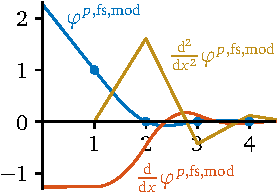
\includegraphics{modifiedFundamentalSpline_1}%
  }%
  \hfill%
  \subcaptionbox{%
    $p = 5$%
  }[48mm]{%
    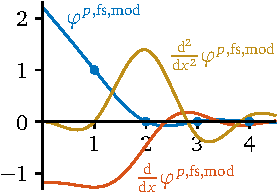
\includegraphics{modifiedFundamentalSpline_2}%
  }%
  \hfill%
  \subcaptionbox{%
    $p = 7$%
  }[48mm]{%
    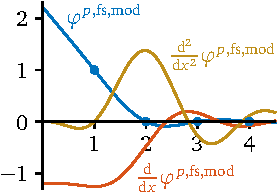
\includegraphics{modifiedFundamentalSpline_3}%
  }%
  \caption[%
    Modified fundamental spline and its derivatives%
  ]{%
    Modified fundamental spline $\parentfundspl[\modified]{p}$
    \emph{\textcolor{C0}{(blue)}} together with its
    first \emph{\textcolor{C1}{(red)}} and
    second \emph{\textcolor{C2}{(brown)}} derivatives
    and the function value interpolation conditions from
    \cref{eq:modifiedFundamentalSplineConditions}
    \emph{\textcolor{C0}{(blue dots)}.}
    For $p = 3$, the second derivative vanishes on
    $\clint{0, 1}$.
    For higher degrees $p > 3$, the second derivative is close to zero
    on this interval, vanishing at $x = 0$.%
  }%
  \label{fig:modifiedFundamentalSpline}%
\end{figure}

\vspace*{\fill}

The conditions stated in \eqref{eq:modifiedFundamentalSplineConditions}
are motivated by the case $p = 3$ of cubic fundamental splines.
The first relevant cardinal B-spline is the one with
index $k = 1 - \tfrac{p+1}{2}$ ($k = -1$ in the cubic case),
as the B-splines with indices $\le -\tfrac{p+1}{2}$ vanish on $\nonnegreal$.
The modified function $\parentfundspl[\modified]{p}$
should satisfy the fundamental property \eqref{eq:tiftDefinition}
at all positive integer points $k \in \nat$.
In contrast to the standard fundamental spline $\parentfundspl{p}$,
we do not enforce the fundamental property at $k = 0$,
as our aim is to obtain non-zero boundary values.
This leaves us exactly two degrees of freedom in the cubic case,
namely $k = -1$ and $k = 0$.
We use these to let $\parentfundspl[\modified]{p}$ extrapolate
linearly on $\clint{0, 1}$, as we did for uniform hierarchical
B-splines (see \cref{sec:313modification}).
\pagebreak
Therefore, in the cubic case, we set the second derivative
$\tderiv[2]{x}{\parentfundspl[\modified]{p}}$ to zero
at $x = 0$ and at $x = 1$.
This suffices since
$\tderiv[2]{x}{\parentfundspl[\modified]{p}}$ is piecewise
linear for $p = 3$.
For higher degrees $p > 3$,
we use the additional degrees of freedom (in total $\tfrac{p+1}{2}$)
to increase the multiplicity of the root of
$\tderiv[2]{x}{\parentfundspl[\modified]{p}}$ at $x = 0$.
This ensures that $\parentfundspl[\modified]{p}$ is
``as linear as possible'' near $x = 0$.
Note that we cannot maintain
$\tderiv[2]{x}{\parentfundspl[\modified]{p}} \equiv 0$
on $\clint{0, 1}$ for higher degrees $p > 3$,
since this would require $p - 1$ conditions,
and we only have $\tfrac{p+1}{2}$ degrees of freedom left,
after taking the fundamental conditions into account.



\subsection{Fundamental Not-A-Knot Splines}
\label{sec:445fundamentalNotAKnotSplines}

The hierarchical fundamental spline basis suffers from the same problem
as the uniform hierarchical B-spline basis.
As explained in \cref{sec:321approximation}, there is a mismatch
of dimensions of the nodal B-spline space $\nsbspl{l}{p}$ of level $l$
when compared with the spline space $\wholesplspace{l}{p}$ on the grid
$\{\gp{l,i} \mid i = 0, \dotsc, 2^l\}$ of level $l$.
This issue also affects the fundamental spline basis.

\paragraph{Definition of fundamental not-a-knot splines}

It is possible to combine the idea of fundamental splines
with the not-a-knot approach from \cref{sec:32notAKnot}.
We define hierarchical fundamental not-a-knot splines
$\bspl[\fs,\nak]{l',i'}{p}\colon \clint{0, 1} \to \real$ as
linear combinations of nodal not-a-knot B-splines of the same level,
where the coefficients are chosen such that the
fundamental property \eqref{eq:fundamentalProperty} is satisfied:
\begin{equation}
  \label{eq:fundamentalNotAKnotSplines}
  \bspl[\fs,\nak]{l',i'}{p}
  \ceq \sum_{i''=0}^{2^{l'}}
  \fundsplcoeff[l',i',\fs]{i''}{p} \bspl[\nak]{l',i''}{p}
  \quad\text{such that}\quad
  \falarge{i = 0, \dotsc, 2^{l'}}{
    \bspl[\fs,\nak]{l',i'}{p}(\gp{l',i}) = \kronecker{i}{i'}
  },
\end{equation}
where $l' \in \natz$, $i' = 0, \dotsc, 2^{l'}$, and
$\fundsplcoeff[l',i',\fs]{i''}{p} \in \real$.
This approach is similar to the \hftr in
\cref{sec:442constructingFundamentalBases},
see \cref{eq:hierarchicalFundamentalTransformation}.
We show the hierarchical fundamental not-a-knot spline basis
of cubic degree in \cref{fig:hierarchicalFundamentalNotAKnotSpline}.

The fundamental not-a-knot splines $\bspl[\fs,\nak]{l',i'}{p}$
of level $l' < \ceil{\log_2(p+1)}$ equal the Lagrange polynomials
$\lagrangepoly{l',i'}$ ($i' = 0, \dotsc, 2^{l'}$),
This is because the $i'$-th summand $\bspl[\nak]{l',i'}{p}$
of \eqref{eq:fundamentalNotAKnotSplines} equals $\lagrangepoly{l',i'}$ and
as $\lagrangepoly{l',i'}$ already fulfills the
fundamental interpolation conditions given in
\eqref{eq:fundamentalNotAKnotSplines}
(see \cref{eq:hierarchicalNotAKnotBSpline}),
we obtain $\fundsplcoeff[l',i',\fs]{i''}{p} = \kronecker{i'}{i''}$, i.e.,
$\bspl[\fs,\nak]{l',i'}{p} = \lagrangepoly{l',i'}$.

\begin{SCfigure}
  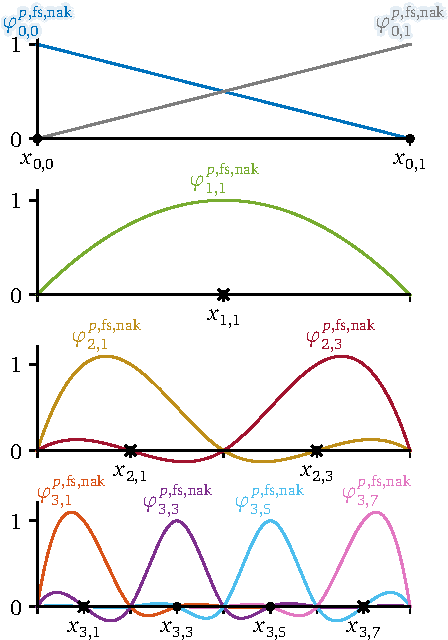
\includegraphics{hierarchicalBasis_16}%
  \caption[%
    Hierarchical fundamental not-a-knot splines%
  ]{%
    Hierarchical cubic fundamental not-a-knot splines
    $\bspl[\fs,\nak]{l',i'}{p}$
    ($l' \le l$, $i' \in \hiset{l'}$, $p = 3$),
    grid points $\gp{l',i'}$ \emph{(dots),} and
    removed knots \emph{(crosses)} up to level $l = 3$.%
  }%
  \label{fig:hierarchicalFundamentalNotAKnotSpline}%
\end{SCfigure}

\paragraph{Implementation}

We make two remarks with respect to the efficient implementation
of hierarchical fundamental not-a-knot splines.
First,
\cref{eq:fundamentalNotAKnotSplines} requires the solution of a system
of linear equations with dimension $2^{l'} + 1$,
which grows exponentially in the level~$l'$.
However, as the coefficients decay roughly in the same order
as the fundamental spline coefficients $\fundsplcoeff{k}{p}$ in
\cref{eq:fundamentalSplineCoefficientsDecay},
we can solve a truncated system of linear equations instead.

Second, the fundamental not-a-knot spline basis
$\bspl[\fs,\nak]{l',i'}{p}$ is not translation-invariant anymore.
This means that theoretically, we have to compute the
$\fundsplcoeff[l',i',\fs]{i''}{p}$ individually for each basis function
$\bspl[\fs,\nak]{l',i'}{p}$.
Nevertheless, when truncating the linear system for a fixed level $l'$,
almost all the inner basis functions $\bspl[\fs,\nak]{l',i'}{p}$
will be identical to hierarchical fundamental splines
$\bspl[\fs]{l',i'}{p}$, if the distance of the region with the removed knots
to the grid point $\gp{l',i'}$ is large enough
(if the removed knots are outside the truncated support of
$\bspl[\fs,\nak]{l',i'}{p}$).
For different levels $l'$, the fundamental not-a-knot splines
$\bspl[\fs,\nak]{l',i'}{p}$ are the same up to scaling
(if the level $l'$ is high enough).

Consequently, an efficient implementation only has to implement
$\bspl[\fs,\nak]{l',i'}{p}$ for some special cases for coarse levels.
The other basis functions can then be derived via an affine
parameter transformation.
